% !TEX root = Projektdokumentation.tex

% 	Die Einleitung soll allgemein verständlich sein, d.h. sie soll beispielsweise auch für Ihre Freunde und Verwandten verständlich sein. Sie stellt die Aufgabe in einen grösseren Zusammenhang und liefert eine genaue Beschreibung der Ausgangslage und Problemstellung. Allfällige Vorarbeiten oder ähnlich gelagerte Arbeiten sind diskutiert. Zum Schluss der Einleitung können Sie auch beschreiben, welche Abschnitte des Berichts sich an welche Leser wenden (z.B. Anwender des Produkts, Entwickler, Betreiber).


%Überprüfen von Wissen \\
Während dem Studium werden viele Inhalte vermittelt und anschliessend mit einer Schlussprüfung abgeholt. Wie merkt ein Student aber schon vor der Prüfung, ob sein Wissen sattelfest ist? Mobile Quiz bietet eine Lösung dafür. Der Dozent publiziert nach jeder Lektion Fragen zu den vorgestellten Inhalten, welche die Studierenden online beantworten können. So erhalten Sie umgehend Feedback zu ihrem Wissensstand.
Die folgende Figur zeigt die wichtigsten Interaktionen der unterschiedlichen Benutzer mit dem Mobile Quiz:

\begin{figure}[H]
	\centering
	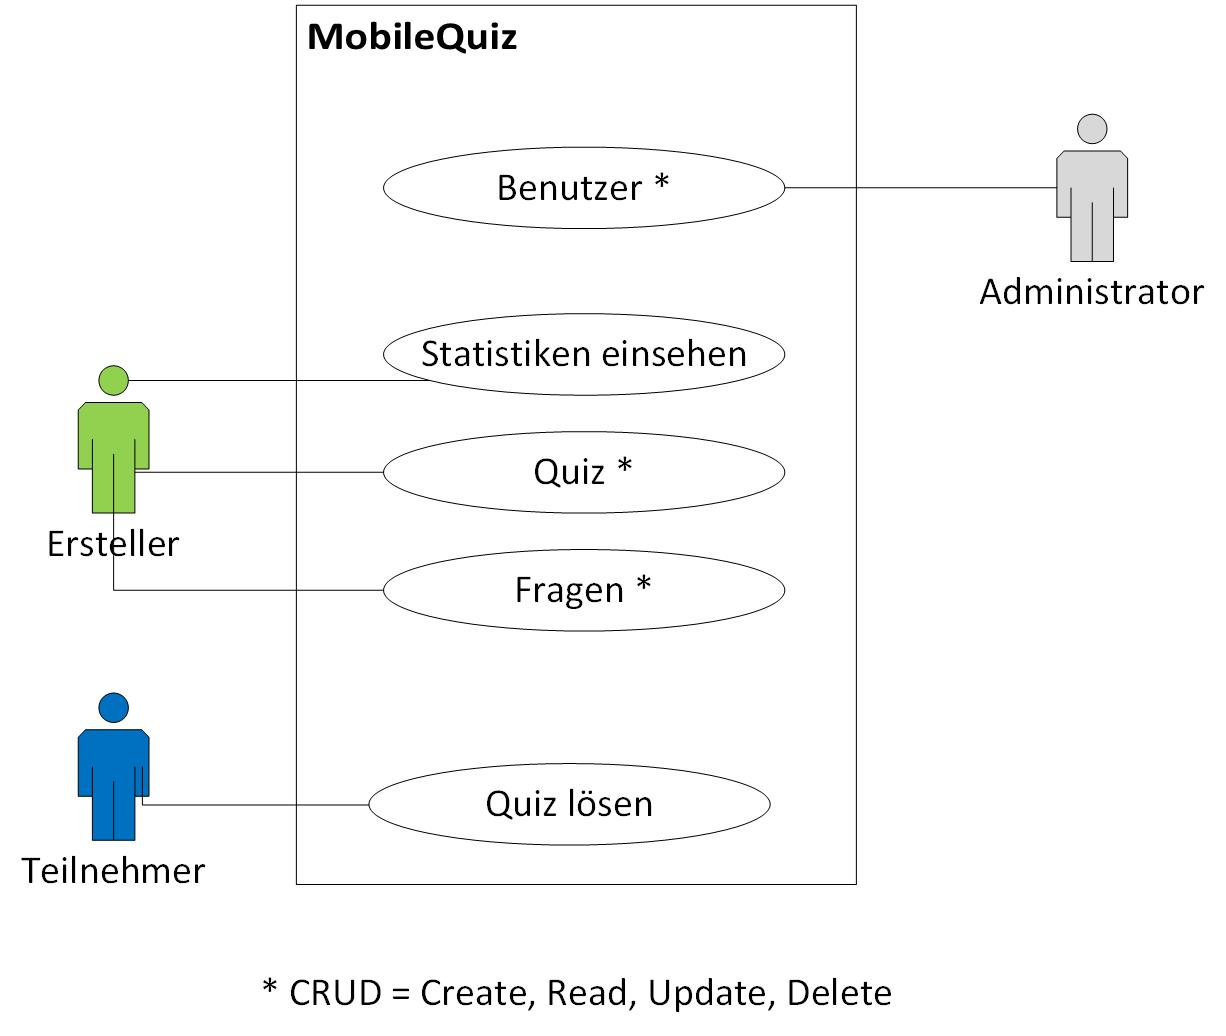
\includegraphics[width=0.75\textwidth]
	{Images/MobileQuiz_Uebersicht.PNG}
	\caption{Übersicht der wichtigsten Funktionen von Mobile Quiz}
\end{figure}

%Stand Mobile Quiz \\
Auf dem Stand vor der Studienarbeit umfasst Mobile Quiz einige Funktionen, um Quizzes zu erstellen. Verbesserungspotentiale liegen allerdings noch in den Bereichen der Bedienbarkeit, im Bereich von neuen Fragetypen sowie in der Auswertung von Quizzes. Durch letzteres wäre es dem Dozenten ersichtlich, welche Teile des Stoffs gut verstanden wurden und bei welchen noch Nachholbedarf herrscht. Somit könnte die Vorlesungszeit effizienter genutzt werden.\\

Die folgenden Bilder zeigen die wichtigsten Ansichten der bestehenden Mobile Quiz - Version. Diese ist unter \url{https://tlng.cnlab.ch/mobilequiz_v3} erreichbar.

\begin{figure}[H]
	\centering
	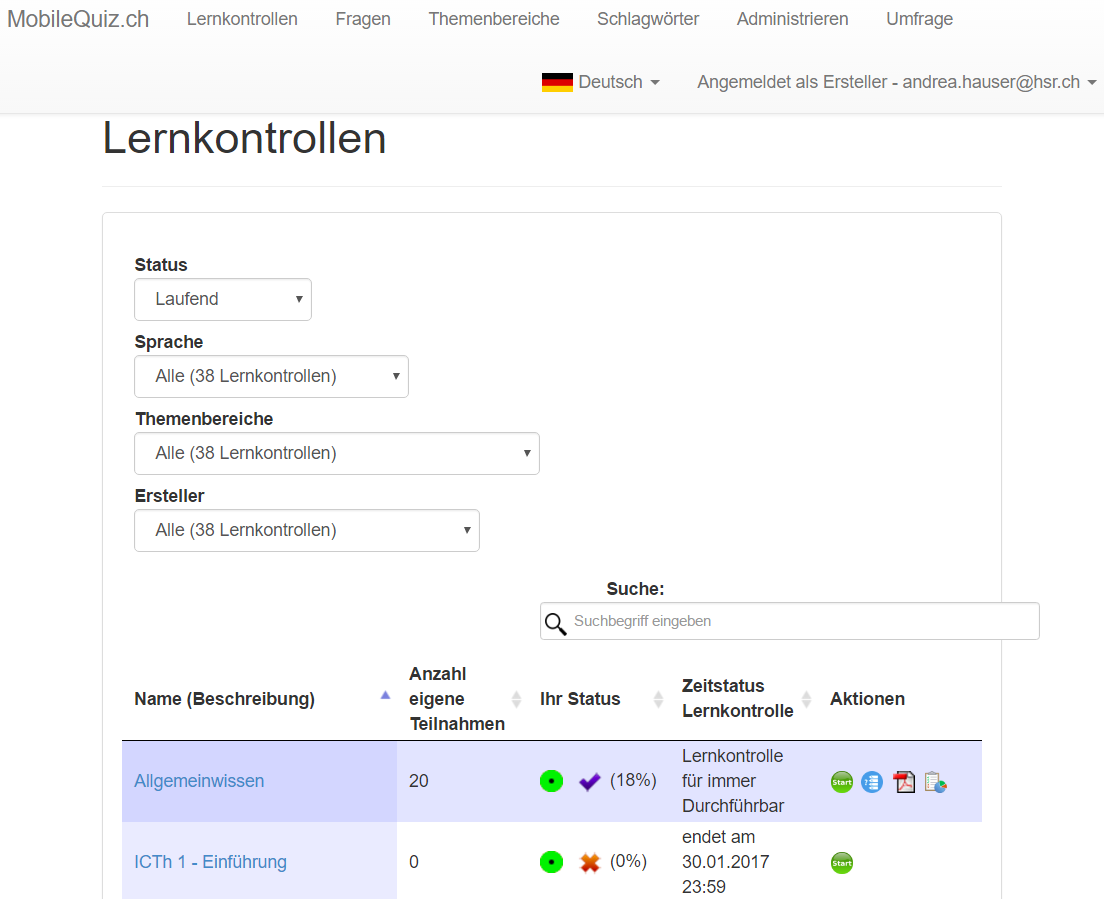
\includegraphics[width=0.75\textwidth]
	{Images/MobileQuizAlteVersionStartseiteErsteller.png}
	\caption{Ansicht der bestehenden Mobile Quiz Startseite}
	\cite{mobilequiz.ch}
\end{figure}

\begin{figure}[H]
	\centering
	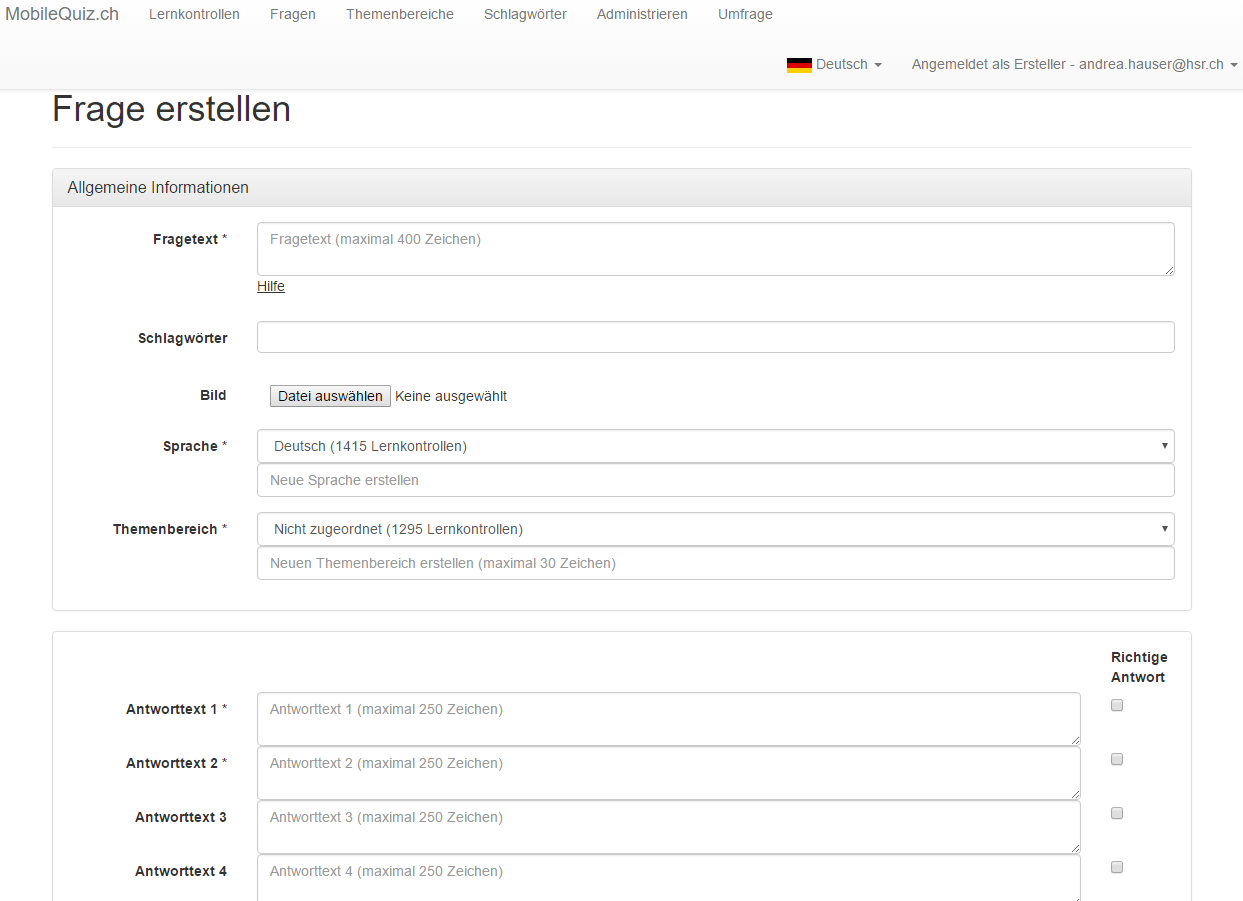
\includegraphics[width=0.75\textwidth]
	{Images/MobileQuizAlteVersionFrageErstellen.png}
	\caption{Ansicht der bestehenden Mobile Quiz Fragen-Erstellungsseite}
	\cite{mobilequiz.ch}
\end{figure}

\begin{figure}[H]
	\centering
	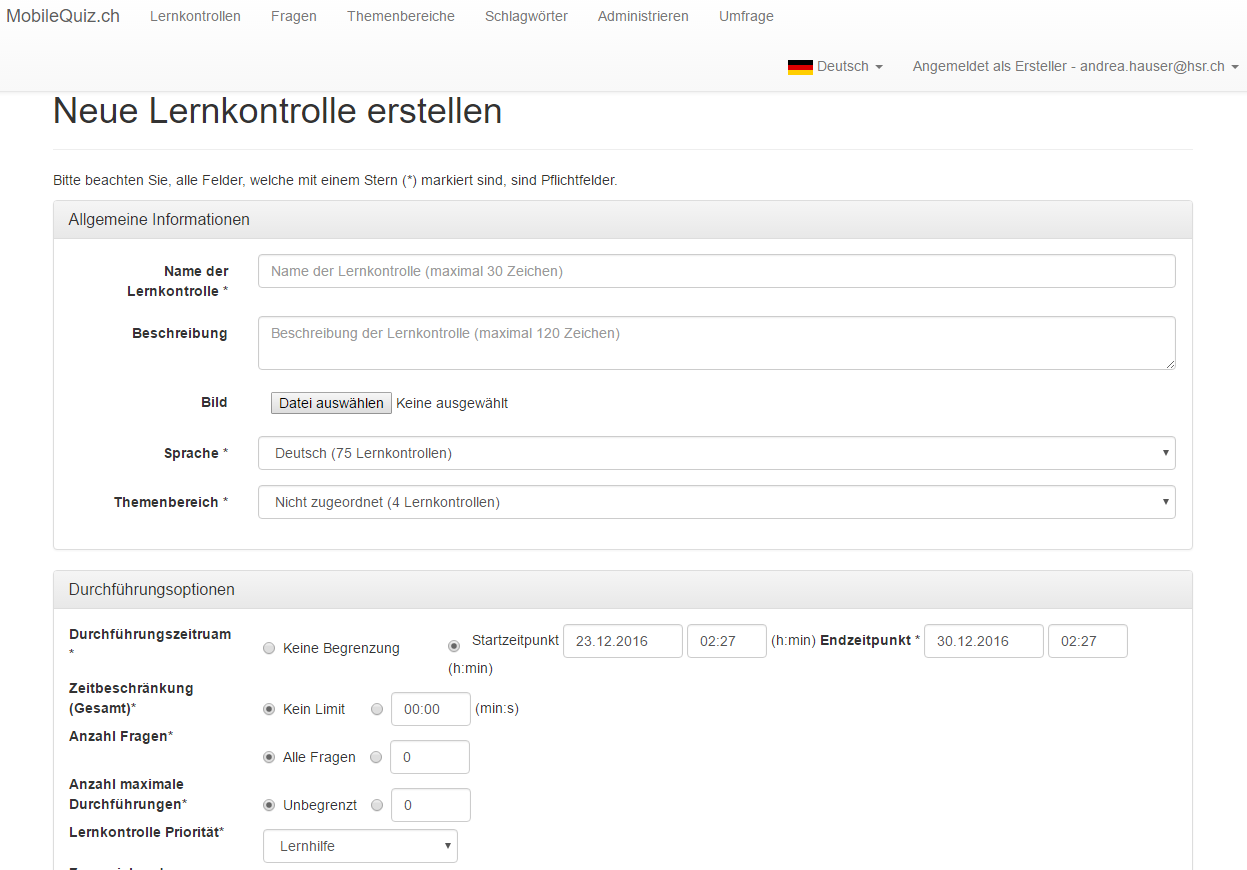
\includegraphics[width=0.75\textwidth]
	{Images/MobileQuizAlteVersionQuizErstellen.png}
	\caption{Ansicht der bestehenden Mobile Quiz Quiz-Erstellungsseite}
	\cite{mobilequiz.ch}
\end{figure}

\begin{figure}[H]
	\centering
	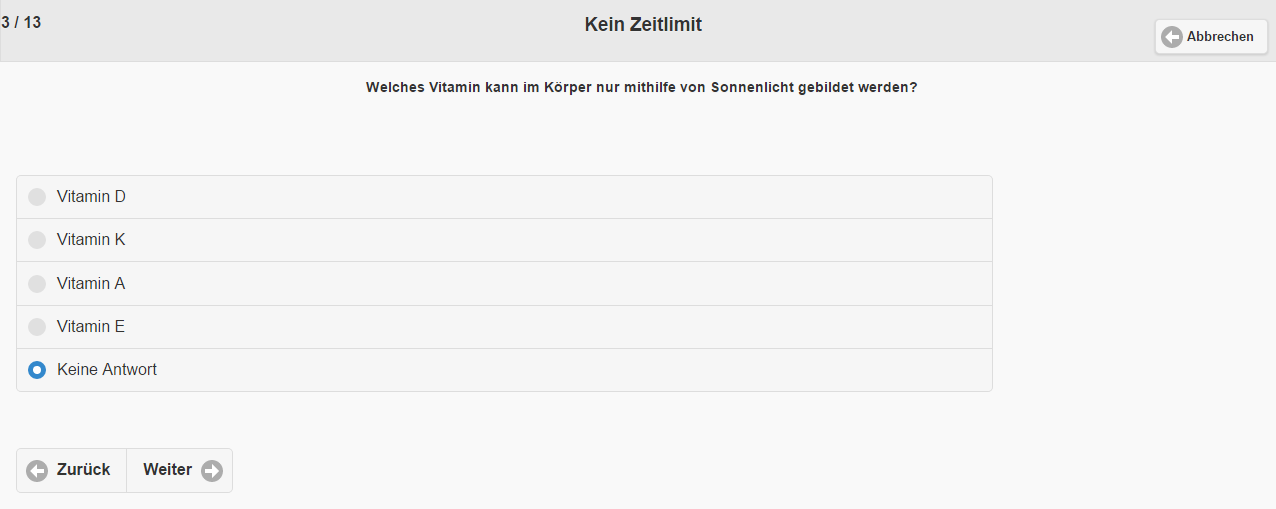
\includegraphics[width=0.75\textwidth]
	{Images/MobileQuizAlteVersionQuizDurchfuehrung.png}
	\caption{Ansicht der bestehenden Mobile Quiz Quiz-Durchführungsseite}
	\cite{mobilequiz.ch}
\end{figure}

%In dieser Arbeit wird XY umgesetzt.
In dieser Arbeit soll eine bessere Bedienbarkeit für Ersteller und Teilnehmer umgesetzt werden. Es wird dabei immer darauf geachtet, dass die Ansichten auch für mobile Geräte bedienbar sind. Zudem werden neue Funktionalitäten, wie zum Beispiel das neue Excel-Template für den Frage-Import oder auch ein neuer Fragetyp implementiert.

\bigskip

%Übersicht Kapitel \\
Im folgenden Kapitel wird das bestehende Produkt genauer beschrieben und es wird darauf eingegangen, wie die Inbetriebnahme ablief. Das Kapitel drei befasst sich mit den zu Beginn vorgenommen Analysen in den Bereichen ähnliche Arbeiten, eigene Tests mit Mobile Quiz und Umfeldanalyse. Im darauf folgenden Kapitel sind die erarbeiteten Konzepte zum Gruppenmanagement, den neuen Fragetypen und den Statistiken und Auswertungen zu finden. Anschliessend folgt das Kapitel Software Engineering in welchem die vorgenommen Datenbankänderungen beschrieben werden. Danach befasst sich das Kapitel sechs mit der Beschreibung der Implementation. Im Kapitel sieben werden die Folgearbeiten beschrieben. Das nächste Kapitel setzt sich mit dem Qualitätsmanagement auseinander. Abgeschlossen wird der Hauptteil mit dem Kapitel Schlussfolgerung.